\chapter{Bioethics: Testing Utilitarianism}

These notes follow a short but sharp continuation of Michael Sandel's \emph{Justice} lectures, in the LazyLearn track curated by LazyingArt LLC with Video2Book. Sandel does not begin by defining utilitarianism in the abstract. He places us inside a role, builds a numerical temptation step by step, and then asks whether the arithmetic settles the moral question. The lecture is brief, but its structure is exact: five urgent needs, no donors, one healthy man, and the pressure of a one-for-five exchange.

\section{Another Doctor Case}

Sandel opens by saying, ``Now consider another doctor case.'' The sense of continuation matters. We are already inside an ongoing examination of moral reasoning, and this new case is introduced not as an essay topic but as a test. The listener is assigned a role immediately: \emph{you} are a transplant surgeon.

The first visual evidence is minimal but useful. It does not show a hospital ward or a surgeon. It shows the count that will govern the case.

\begin{figure}[h]
\centering

\includegraphics[width=0.72\textwidth]{lecture_14_figure_01.png}
\end{figure}

A nearby redraw can remain equally spare. Its function is simply to preserve the fivefold symmetry of the patients without importing extra notation that is not visible in the frame.

\begin{figure}[h]
\centering
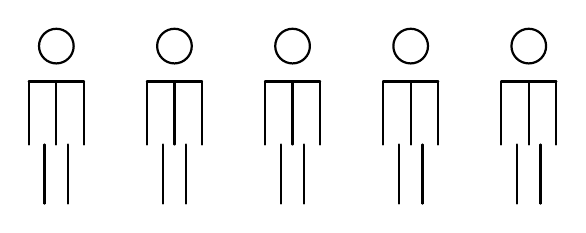
\begin{tikzpicture}[x=1cm,y=1cm,line cap=round,line join=round, thick]
\foreach \x in {0,1.5,3.0,4.5,6.0}{
  \draw (\x,2.0) circle (0.22);
  \draw (\x-0.35,1.55) -- (\x-0.35,0.75);
  \draw (\x+0.35,1.55) -- (\x+0.35,0.75);
  \draw (\x-0.35,1.55) -- (\x+0.35,1.55);
  \draw (\x,1.55) -- (\x,0.75);
  \draw (\x-0.15,0.75) -- (\x-0.15,0.0);
  \draw (\x+0.15,0.75) -- (\x+0.15,0.0);
}
\end{tikzpicture}
\end{figure}

The frame itself contains no visible notation, but a compact summary of what it contributes is
\begin{equation}
N_{\text{patients}} = 5.
\end{equation}
This is our editorial shorthand, not something written on screen. Still, it captures the structural role of the figure exactly.

\subsection{Question \& Answer}

\paragraph{Question.} At the start of the case, what is morally salient: five separate persons, or one aggregate need of size five?

\paragraph{Answer.} Sandel makes us hold both at once. The image gives us a count, but the lecture immediately resists any simple flattening of the five into a mere number by specifying what each of them needs. The case begins in aggregation, but it does not stay there.

\section{Five Organs, No Donors}

The next move is to individualize the patients medically without dissolving the aggregate structure. One needs a heart, one a lung, one a kidney, one a liver, and the fifth a pancreas. Sandel slows the case down just enough for us to feel that there are five distinct people here, not merely five interchangeable units.

A clean way to write the setup is
\begin{align}
N_{\text{patients}} &= 5,\\
\text{needed organs} &= \{\text{heart},\ \text{lung},\ \text{kidney},\ \text{liver},\ \text{pancreas}\},\\
N_{\text{donors}} &= 0.
\end{align}
The last line does the real work. There are no organ donors. The ordinary path out of the problem has been removed.

So the case tightens into the following implication:
\begin{equation}
N_{\text{donors}} = 0
\Longrightarrow
\text{without intervention, all five patients die}.
\end{equation}
This is where Sandel turns a sad medical situation into a genuine dilemma. The five are not merely in danger; they are about to die, and there is no available donor source within ordinary medical practice.

\section{The Healthy Man in the Next Room}

Only after the scarcity condition is fixed does the decisive pivot arrive. It occurs to the surgeon that in the next room there is a healthy man who came in for a checkup. The transcript is noisy for a few seconds around this point, but the stable structure is clear enough: there is one healthy person nearby, apparently asleep, whose organs could in principle supply the needs of the five.

The new count is therefore
\begin{equation}
N_{\text{healthy candidates}} = 1.
\end{equation}
This changes the moral geometry of the case. We are no longer facing simple tragedy. We are facing a possible act of sacrifice.

Sandel's proposal can be written with brutal economy:
\begin{equation}
\text{save }5\text{ by sacrificing }1.
\end{equation}
And that compact formula matters because it marks the exact point at which the case stops being purely descriptive. Once one healthy person is present as a possible source of the five organs, the surgeon is tempted to convert scarcity into an act of intentional killing.

\subsection{Question \& Answer}

\paragraph{Question.} Does the appearance of one healthy person make the five-to-one trade morally available?

\paragraph{Answer.} It makes the trade thinkable, and that is enough for Sandel's immediate purpose. The lecture is testing whether numerical advantage alone can authorize the act. At this stage the issue is opened, not yet closed.

\section{The Utilitarian Arithmetic Under Test}

Here the mathematical spine of the lecture comes into view. If we count lives symmetrically, then the attraction of the case is obvious:
\begin{equation}
5 > 1.
\end{equation}
That is not Sandel's verdict. It is the temptation he has built into the scenario.

We can state the same temptation more explicitly as a worked count:
\begin{align}
\text{do nothing} &\Longrightarrow 5 \text{ deaths},\\
\text{kill }1\text{ healthy man and distribute organs} &\Longrightarrow 1 \text{ death and }5 \text{ survivals},\\
\Delta N_{\text{lives}} &= 5 - 1 = 4.
\end{align}
Again, this is our compact reconstruction of the structure, not a literal board derivation from the lecture. But it captures exactly what Sandel wants the audience to feel: on a purely aggregative view, the proposed act appears to generate a positive surplus.

We can make the utilitarian rule under examination fully explicit:
\begin{equation}
\text{maximize lives saved}
\Longrightarrow
\text{kill }1\text{, save }5.
\end{equation}

\paragraph{Worked example.} The numerical reasoning proceeds in a few short steps:
\begin{enumerate}
\item Without intervention, the five patients die.
\item The healthy man supplies the five needed organs.
\item If one life may be traded against five, the act saves more lives than it destroys.
\item Therefore a simple maximizing rule points toward killing the one healthy man.
\end{enumerate}
What Sandel is testing is whether this derivation, sound as a piece of counting, is also sound as a moral argument.

\subsection{Question \& Answer}

\paragraph{Question.} If the arithmetic points toward killing one to save five, what exactly is left to object to?

\paragraph{Answer.} The open question is whether morality can be exhausted by aggregation. Sandel's construction forces us to ask whether the healthy man is merely one term in a sum, or a person whom the surgeon may not use in this way even for the sake of producing a better total outcome.

\section{Would You Do It?}

The lecture does not end this opening movement by offering a theorem. It ends by turning the case back on the audience. After the proposal has been made concrete, Sandel asks, ``How many would do it?'' The laughter around the setup matters. It marks the room's recognition that the arithmetic, once converted into action, demands something morally extreme.

The final fork of the case can be written in the plainest possible form:
\begin{equation}
\text{kill }1\text{, save }5
\qquad \text{or} \qquad
\text{refuse to kill and let }5\text{ die}.
\end{equation}
That is why the case is so effective as a test. Both branches carry death. The left-hand side minimizes deaths in the aggregate. The right-hand side refuses to make the surgeon the deliberate killer of an innocent patient. Sandel does not resolve the tension for the audience at this moment; he makes them inhabit it.

\subsection{Question \& Answer}

\paragraph{Question.} If the count favors one branch, why do many listeners still resist it?

\paragraph{Answer.} Because the lecture has been designed to expose a gap between what counting recommends and what moral agency can comfortably endorse. Sandel is not merely asking for a calculation. He is asking whether a surgeon may intentionally kill an innocent person in order to improve the total outcome.

\section{Summary}

Sandel's transplant-surgeon case is constructed with unusual precision. First we are given five patients, then five distinct organ needs, then the elimination of all ordinary donors, then one healthy man in the next room, and only then the proposal to kill one in order to save five. The arithmetic is simple enough to write as
\begin{equation}
\Delta N_{\text{lives}} = 5 - 1 = 4,
\end{equation}
but the whole force of the lecture lies in the possibility that the moral truth of the case is not exhausted by that arithmetic.

This is what makes the example a serious test of utilitarian reasoning. It lets the maximizing argument appear in its strongest local form, and then asks whether we are prepared to live by it once the numbers are attached to an actual human act.